% What のみを書く - Why はイントロへ
\section{Background}
まず、単一のエージェントが PODMP 環境で行動する場合について考える。
POMDP 環境とは 7 つ組 $(\S, \A, \Trans, \R, \Observations, \ObProb, \gamma)$ である。
ただし、$\S$は状態集合、$\A$ は行動集合、$\Trans$ は遷移確率、$\Observations$ は取りうる観測の集合、$\ObProb$ は観測の集合、$\gamma$ は減衰率である。
エージェントは観測 $o \in \Observations$ を通して部分的に状態 $\S$ を推定する。
一般に $o$ の方が $s$ よりも次元が大きく、複雑である。
たとえば、Atari 2600 は真の状態である RAM は 128 バイトしかないが、そこから生成される画像 $o$ は 10,000 以上の次元を持っている。
そのため、DQN や DRQN では、$o$ の情報を抽象化し、独自の状態表現を作っていると解釈できる(DQN の原著論文では MDP であることを前提としているが、DRQN の論文で環境が POMDP であることが主張されている)。
もちろん、DQN はモデルフリーの手法であるため、直接は状態遷移を扱わないが、出力層の一個手前の層に状態が格納されているという解釈もできる\citep{zahavy2016graying}。
以下では、エージェントはニューラルネットワークを通して行動を決定することを前提とする。

次に、互いに通信するマルチエージェントシステムを考える。
一般にエージェントが多いほど、観測を増やすことが可能である。
たとえば、自動運転のケースでは自動車同士が通信することでより正確な世界に対する知識を得ることができる。
この時、エージェントが持っているニューラルネットワーク同士をつなげる方法がとられている\citep{sukhbaatar2016learning}。
これは、マルチエージェントシステム全体を一つのニューラルネットワークをとらえることができると考えられる。
そこで、本研究ではこれを拡張し、すべてのユニットをエージェントとみなす。
%すなわち、ニューラルネットワークにおける各ユニットをエージェントとみなした場合の、最適化を行う。

%以下では、ニューラルネットワークとは広義の
%DRQN では隠れた状態の推定はニューラルネットワークを使って行われることが多い。
%リバースエンジニアリングしていると解釈できる。


\section{Neuron as an Agent}
ニューラルネットワークを、ユニット間の有向グラフ $\neuralnet = (\units, \edges)$で表す。
$\units = \{\unitAt{1}, \dots, \unitAt{N}\}$ はユニットの集合であり、$\edges \subset \units^2$ はユニットの接続関係を表すエッジの集合である。
$(\unit, \unitAt{j}) \in \edges$ であるとき、$\unit \rightarrow \unitAt{j}$ という接続関係が成立し、$\unitAt{j}$ は $\unit$ から値を入力する。
ユニットの $\unit$ の時刻 $t$ における出力を $x_{it} \in \Real$ で表す。
ユニット $i$ の出力先の集合を $\followers = \{j | (\unit, \unitAt{j}) \in \edges \}$、n入力元の集合を $\followees = \{j | (\unitAt{j}, \unit) \in \edges \}$ で表現する。
$\friends = \followees \cup \followers$ とする。

NaaA は $\unit$ をエージェントとしてとらえる。すなわち、$\neuralnet$ はマルチエージェントシステムである。
$\unit$ にとっての環境は、マルチエージェントシステムの自体が触れている環境と、$\unit$ が直絶接続しているユニット群 $\{v_i \in V | i \in \friends\}$ である。
前者を外的環境(external environment)、後者を内的環境(internal environment)と呼んで区別する。
$\unit$ は環境から報酬を受け取る。
$\unit$ の性質として以下の前提を加える。
\begin{enumerate}
\renewcommand{\labelenumi}{N\arabic{enumi}:}
\item (利己性)$\unit$ は、各時点 $t$ において、汎化誤差の最小化ではなく、自身のリターン(累積減衰報酬)$G_{it} = \sum_{i=0}^T \gamma^i \rewardAt{i,t+k} $ の最大化を目的として行動する。ただし $\gamma \in [0, 1]$ は減衰率(discount rate)、$T$ は終端時間である。
\item (保存則)$\unit$ が環境から受け取る報酬 $\reward$ の総和は、マルチユニットシステム全体が外的環境から得る報酬 $R_0$ に等しい。
\item (取引)$\unit$ は信号 $x_i$ を $\unitAt{j} \in \units$ に伝達する際に、信号と引き換えに報酬 $\rho_{jit}$ を受け取る。
\item (NOOP)$\unit$ は、期待リターンが 0 の NOOP (no operation) という行動をオプションとして持つ。NOOP では、ユニットは何も入力せず、何も出力しない。
\end{enumerate}
N1 はユニットがエージェントとして振る舞うことを述べている。
N2, N3 は NTF の分配に、N4 はニューロンのアポトーシスに相当する。
NOOP が選択されるのは、それ以外のすべての行動の期待報酬が負であった場合である。
以下ではこれらの前提から出発して、NaaA の仕組みを構築していく。

\subsection{Cumulative Discounted Profit Maximization Framework}
%NaaA では、すべてのユニットがエージェントとしてパラメータの最適化を行う。
%接続されている入力元、出力先のユニットは、環境の一つとして扱われる。
%ユニットは他のユニットから報酬を受け取ったり、支払ったりする。
%
%%N2, N3 より、報酬はマルチエージェントシステムに対して支払われる $R_0$ は、フローとしてニューラルネットワーク上を流れる。
%そこで、通貨のメタファーを用いて、$R_0$ を分解しながら他のニューロンに対して伝達することを考える。
%ユニットは、他のユニットから受け取る報酬と、他のユニットに対して支払う報酬の差が報酬となる。
%前者を収益(reward)、後者をコスト(cost)と呼び、その差を利益(profit)と呼ぶ。

ユニット $i$ が時刻 $t$ で外部から得る報酬を $R_i^\mathrm{ex}$ と書き、消費エネルギーを $\alpha_{it}$ で表す。
時刻 $t$ に $i$ が獲得する報酬 $R_i$ は次のように表現される。
\begin{flalign}
	R_{it} = 
	  \left[ R_{it}^\mathrm{ex} + \sum_{j \in N^\mathrm{out}_i} \rho_{jit} \right] 
	- \left[\sum_{j \in N^\mathrm{in}_i} \rho_{ijt} + \alpha_{it} \right]
\end{flalign}
この式は、符号が正の項と負の項の二つに分解される。前者を収益(revenue)、後者をコスト(cost)と呼び、それぞれ $r_{it}, c_{it}$ で表す。$R_{it}$を利益(profit)と呼ぶ。
%今、外的環境を $\unitAt{0}$ と書き、$\rho_{0it} = R_{it}^\mathrm{ex}$, $\rho_{i0t} = \alpha_t$ と書くと、この式は次のように単純化される。
%\begin{flalign}
%	R_{it} 
%	&= \sum_{j \in N^\mathrm{out}_i \cup \{0\}} \rho_{jit} - \sum_{j \in N^\mathrm{in}_i \cup \{0\}} \rho_{ijt} 
%	%&= (\mathbf{J} - \mathbf{J}^\T) \mathbf{R}
%\end{flalign}
%%ただし、$\mathbf{J}$ は $\edges$ の隣接行列であり、$(i,j)$-要素の値は $(\unit, \unitAt{j}) \in \edges$ であるときに 1 であり、それ以外は 0 である。
%
%
%今、$\vect{r}_t= (r_{1t}, \dots, r_{nt}), \vect{R}_t = (\rho_{ijt})_{ij}$ と表現すると、次のように書くことができる。
%\begin{flalign}
%	\vect{r}_t = \left( \vect{R}_t - \vect{R}_t^\T \right) \vect{1}
%\end{flalign}
%ただし、$\vect{1}$は要素がすべて $1$ のベクトルである。
%
%リターンは次のように書くことができる。
%\begin{flalign}
%	\vect{y}_t = \sum_{i=0}^T \gamma^i \vect{r}_{t+i}
%\end{flalign}
%ただし、$T$ は終端時間である。

このとき、ユニット $\unit$ は、次式で表現される累積減衰利益 $G_{it}$ を最大化する。
\begin{flalign}
	G_{it} = \sum_{k=0}^T \gamma^k R_{i, t+k} = \sum_{k=0}^T \gamma^k (r_{i,t+k} - c_{i,t+k})
\end{flalign}
$R_{it} > 0$、すなわち、$r_{it} > c_{it}$ であれば、ユニットは得たデータに対して付加価値を与えていることになる。
もし、すべての $t$ に対して $R_{it} < 0$ であれば、$G_{it} < 0$ であるから、ユニットは NOOP になる。

%ユニットは、得た報酬を他のユニットに対してどのように分配するのかに関する方策 $\pi$ を持つ。
%強化学習と同様に以下の目的関数を持つ。
%\begin{flalign}
%\Expect{\pi}{\sum_{i=0}^{T} \gamma^i (r_{t+i} - c_{t+i})}
%&= \Expect{\pi}{\sum_{i=0}^{T} \gamma^i r_{t+i}} -  \Expect{\pi}{\sum_{i=0}^{T} \gamma^ic_{t+i}} \notag \\
%&= G_t^{\mathrm{in}} - G_t^{\mathrm{out}}
%\end{flalign}
%ただし、$G_t^{\mathrm{in}} \equiv \Expect{\pi}{\sum_{i=0}^{T} \gamma^i r_{t+i}}$、
%$G_t^{\mathrm{out}} \equiv \Expect{\pi}{\sum_{i=0}^{T} \gamma^ic_{t+i}}$ である。
%この式は、エージェントが終端状態までに生み出した付加価値に等しい。
%これを行うために、エージェントは収益の最大化とコストの最小化を同時に行うことがわかる。
%

\section{Optimization}
%ここでは、NaaA のフレームワークにおいて、ニューラルネットワークを最適化する手法について説明する。
%最適化の方法はいくつかあるが、practical な方法として、envy-free auction と valuation net の二つを紹介する。
%
NaaA では利益を最大化するため、二つの相反する指標である収益 $r_{it}$ とコスト $c_{it}$ のバランスを取ることが重要になる。
本研究では、この最適化にゲーム理論の一つであるメカニズムデザインを応用する。
メカニズムデザインは、マルチエージェントシステムを対象にしたゲーム理論の分野であり、各エージェントが利己的であることを想定した上で、システム全体が最適になるような帰結を目指すメカニズムの設計を目的とするものである。

メカニズムデザインを導入する理由は、NaaA いくつかの既存研究と異なり、すべてのエージェントが協力的ではなく、利己的であると仮定していることに起因している。
前述の問題は、そのまま最適化すると報酬額は 0 に収束するため、すべてのニューロンが NOOP になるという trivial な解が得られる。
%すなわち、単純な累積利益最大化フレームワークでは、すべてのニューロンが活動せず、
マルチエージェントシステムは無情報でアクションを選択する必要が生じ、これはランダムなアクションを取っている状況に等しい。
したがって、明らかに外的環境からの報酬 $R_t$ は小さくなる。

このように最適化を行った結果、システム全体が最適化されない現象はジレンマとして知られており、囚人のジレンマ問題をはじめとし様々な研究が行われている。
しかし、一般にエージェントが利己的であると仮定した場合の最適化は難しいとされている。
メカニズムデザインはこうした問題を解決することができる。

%NaaA のフレームワークを最適化する方法について述べる。
%残念ながら、前述の問題に対しては以下の否定的な解が得られる。
%
%%実際には、このフレームワークは期待通りに動作しない。
%%なぜなら、この式を最適化すると、コスト最小化によってエージェントは他のエージェントに対して金額を支払わないことがナッシュ均衡解として得られるためである。
%%
%\begin{thm}\label{thm:optimal-bidding-simple}
%	The Nash equivalem of the game $(r_{ijt})$ is $0$.
%\end{thm}
%ただちに、次の系が成立する。
%\begin{coro}\label{coro:optimal-bidding-simple}
%NaaA では、外的環境から報酬を受け取らないニューロンはすべて NOOP になる。
%\end{coro}


%これは、ナッシュ均衡がパレート最適と一致しないパレート劣位な状況が発生する。


\subsection{Envy-free Auction}
パレート効率な仕組みを作るために、我々はオークション理論における digital goods auction からアイデアを借りる。
オークション理論は、ゲーム理論におけるメカニズムデザインという分野に属しており、
複数のエージェントの利害を一致させ、全体としてパレート最適を目指すことを目指している。
digital goods auction は、本や音楽などの、複製可能な財を割り当てる仕組みを作っている。

Digital goods auction にはいくつかバリエーションがあるが、
本研究では単純な前提のみを設けるだけでよいという理由から envy-free auction \citep{guruswami2005profit} を用いる。
これは、同じ時点取引において、一つのユニットの価格を同じにするというものである。
NaaA において、これは次の前提によって表現できる。
\begin{enumerate}
\renewcommand{\labelenumi}{N\arabic{enumi}:}
\setcounter{enumi}{4}
\item (一物一価)
	$\rho_{j_1,i,t}, \rho_{j_2,i,t} > 0$ であれば $\rho_{j_1,i,t} = \rho_{j_2,i,t}$ 
\end{enumerate}
これは、ユニット $\unit$ は同じ時間(timing) $t$ に個有の価格を持つことを意味する。
この価格を $q_{it}$ で表す。

\begin{figure*}[t]
\centering
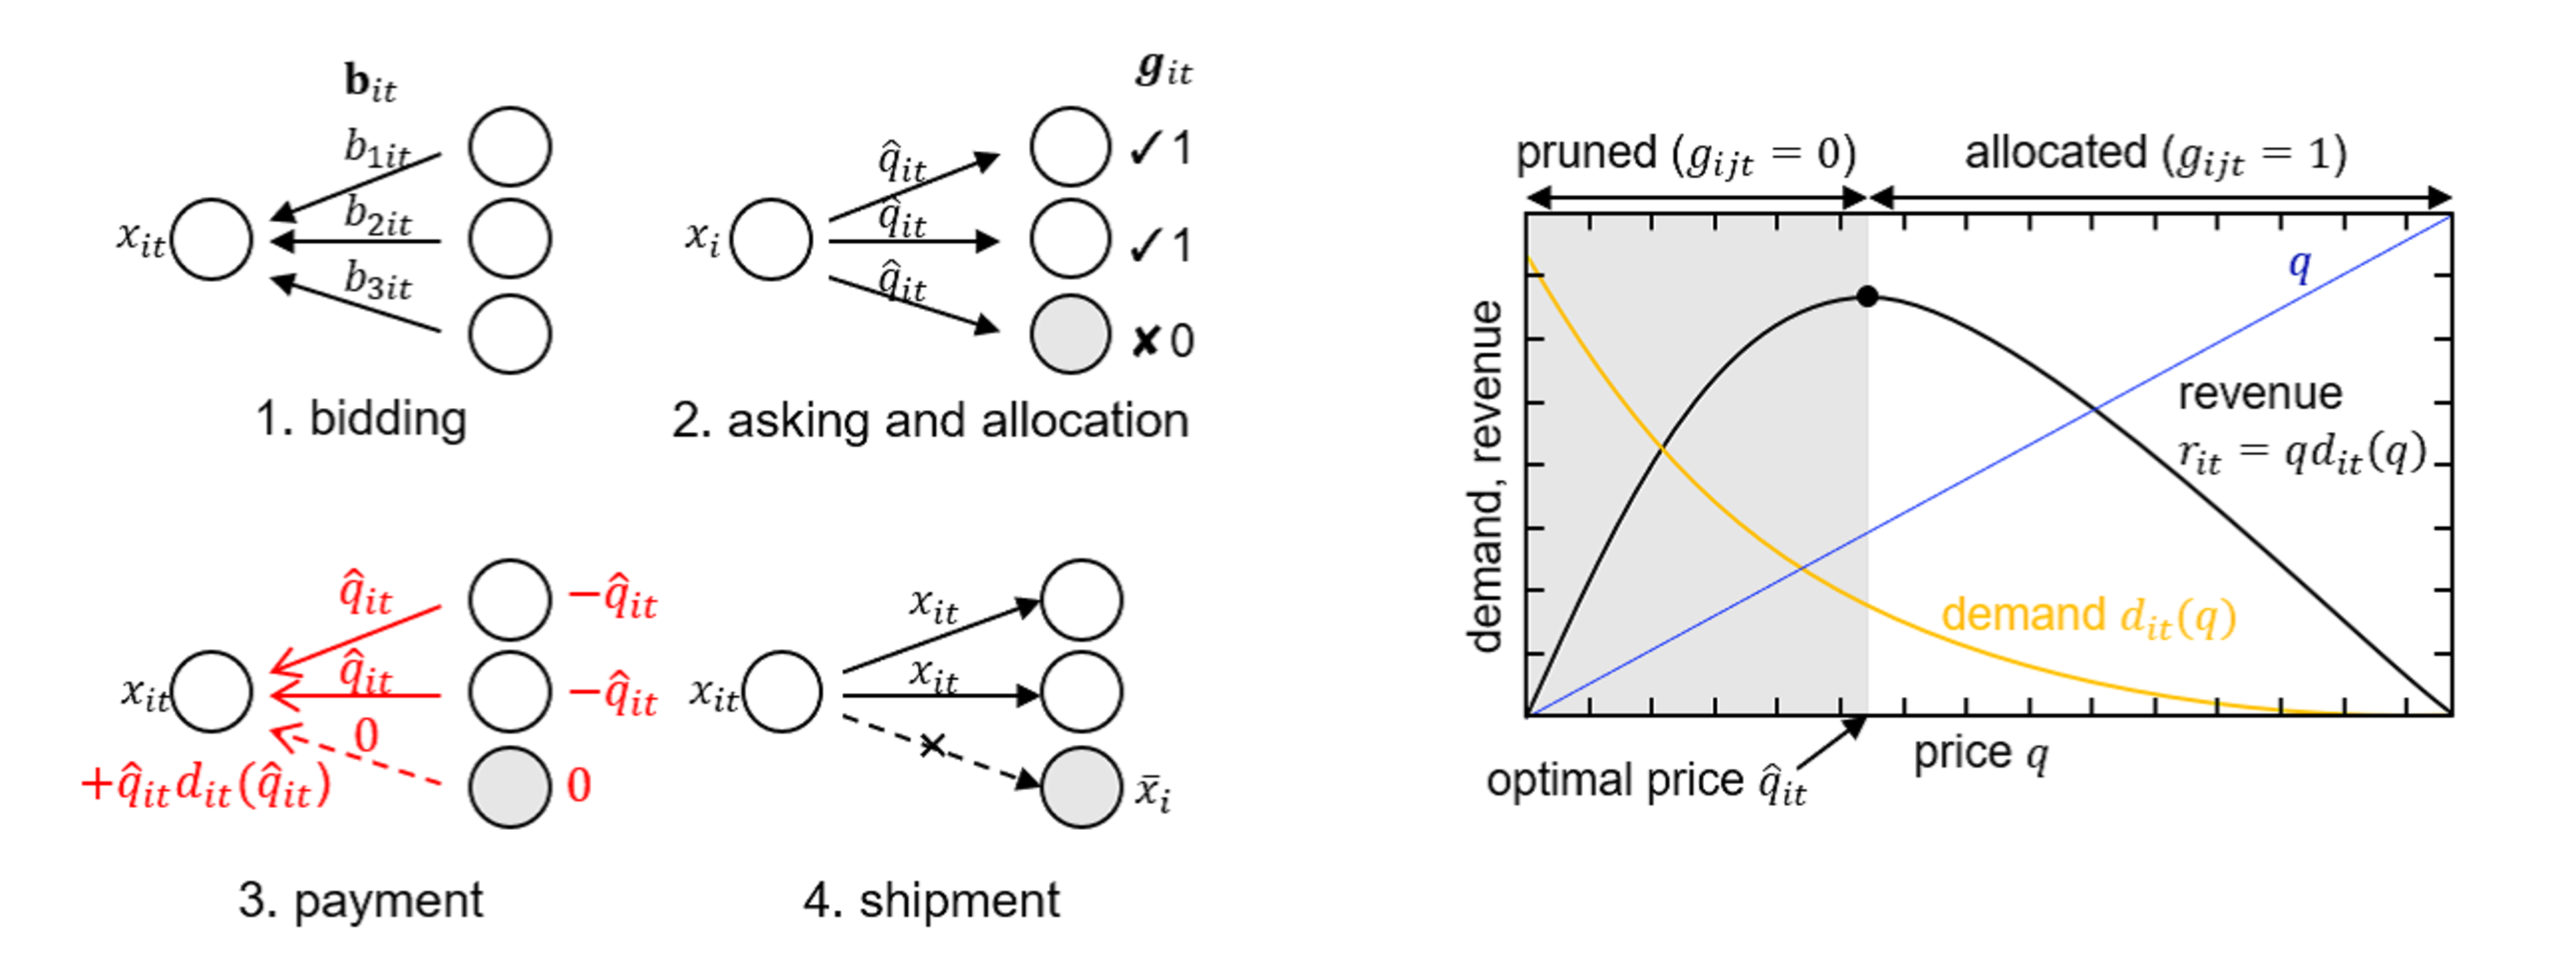
\includegraphics[width=\linewidth]{img/double.eps}
\caption{
Left: NaaA による取引の流れ。
Right: ユニットの価格決定方法。ユニットの収益は単調減少な需要と価格の積となり、これを最大化する価格が最適価格となる。
}
\label{fig:double}
\end{figure*}

% TODO 割当の話
Envy-free auction の流れを Figure \ref{fig:double} の左に示す。
図は、信号を送信する一つのユニットと、その信号を「購入」する複数のユニットに分かれ、交渉の過程を示している。
一単位の交渉は、強化学習の時間軸では 1 ステップ内に完了し、これが複数回繰り返されることになる。
信号を送信する側を売り手、受信する側を買い手と呼ぶ。
買い手はユニットに対して入札 $b_{jit}$ を行う(1)。次に、入札額をもとに、売り手は価格 $\opt{q}_{it}$ を決定し、割当を行う(2)。
このとき、$b_{jit} \ge \opt{q}_{it}$ であれば割当を行って $g_{jit} = 1$ とし、そうでなければ $g_{jit} = 0$ とする。
割当を行った後は、$\rho_{jit} = g_{jit} \opt{q}_{it}$ として、送金を行い(3)、
売り手は割当を行ったノードに対してのみ信号 $x_i$ を送付する(4)。
信号を受け取れなかったノードは、$x_i$ の期待値 $\Expect{\pi}{x_i}$ によって $x_i$ を近似する。
以下では、Envy-free auction における収益 $r_{it}$ とコスト $c_{it}$ の最適化について分けて説明を行う。

%この過程は、本や音楽などの、複製可能財、digital goods を対象にしたオークション理論 digital goods auction において、
%envy-free auction として知られている。
%後で示すように、このシンプルな前提のみでジレンマの問題が解決する。
%NaaA による取引の流れを図\ref{fig:double}に示す。

%========================================
% 収益
%========================================

\textbf{Revenue}:
エージェントの収益は次式で与えられる。
\begin{flalign}
	r_{it}  &= \sum_{j \in N^\mathrm{in}_i} g(b_{jit}, q_i) q_i + R^\mathrm{ex}_i  = q_i \sum_{j \in N^\mathrm{in}_i} g(b_{ji}, q_i)  + R^\mathrm{ex}_i \notag \\
		&= q_i d_t(q_t) + R^\mathrm{ex}_i
\end{flalign}
ここで、$a$ は価格、$d_t(a)$ はユニット $i$ の信号に対する価値を $a$ 以上と評価しているエージェントの数であり、需要(demand)と呼ぶ。
同様の式で、右辺を最大化する $a$ を最適価格と呼び、$ \opt{q}_{it} $ で表す。 
第二項は $q_t$ に対して独立であるから、最適価格 $\opt{q}_{it}$ は次のようにして与えられる。
\begin{flalign}
	\opt{q}_{it}  = \argmax_{q \in [0, \infty)} q d_{it}(q)
\end{flalign}
この仕組みを、Figure \ref{fig:double} の右に図示する。$d_t(q_{it})$ は単調減少な関数であり、$q_{it}$ との積によって表現される。


%========================================
% コスト
%========================================

\textbf{Cost}:
コストは、正しいデータを購入した場合とそうでない場合の期待リターン $G_{it}$ の差に等しい。
すなわち、
%FIXME 多分ここは期待値じゃなくてリターンそのものなのでそのように修正する(最初にリターンを使ったロジックで説明しているため)
\begin{flalign}
	o_t 
	&= \Expect{\pi}{ r_{i,t+1} \mid a_t=1 } - \Expect{\pi}{ r_{i,t+1} \mid a_t=0 } \notag \\
	&= \Expect{\pi}{ R_{i,t+1} \mid a_t=1 } - \Expect{\pi}{ R_{i,t+1} \mid a_t=0 } \notag \\
	&= Q(s_t, 1) - Q(s_t, 0) \label{eq:def:oppotunity-cost},
\end{flalign}
ただし、$Q$ は状態行動価値関数であり、一手先のコストはどちらの行動を選んでも一定であると仮定している。
$o_{it}$ を counterfractual state-action value と呼ぶ。これは QUICR \citep{agogino2006quicr} と導出は異なるが等価である。
すなわち、エージェントが支払うコストは、データの購入に成功した場合は $\opt{a}_{it}$ であり、
それ以外は $o_{it}$ となる。

では、コストを最小化するためのエージェントの入札額 $b_{it}$ は何か。
これについては次の定理が成立する。

\begin{thm}\label{thm:optimal-bidding}
コストを最小化する最適な入札額は $b_{it} = o_{it}$ である。
\end{thm}
証明については Appendix を参照。

すなわち、エージェントは自身の機会損失のみを問題にすればよい(!)
したがって、NaaA のメカニズムでは、エージェントはあたかも他のエージェントを価値評価(valuation)し、
その価値を正直に申告していることを意味する。

系として次の解が得られる。
\begin{coro}\label{coro:optimal-bidding}
The Nash equivalem of the envy-free game $(\vect{b}, q)$ is $(\vect{o}_t, \max_{q} q d_{\vect{o}_t}(q))$.
\end{coro}

%TODO o_t のグラウンドをする。最初に望ましい配分 v を述べ、その後で重要性について解説する。


\subsection{Valuation Net}

\begin{figure*}[t]
\centering
\includegraphics[width=\linewidth]{img/network.eps}
\caption{
Valuationn Net は情報の価値を評価し、bidding price を決定する。
下位のニューロンに対して入札し、信号を購入する。購入したデータを用いて、データを次のニューロンに対して売る。
}
\label{fig:network}
\end{figure*}

残る問題は、$\vect{o}_t$ をいかに推定するかである。
この推定には様々な方法が存在しており、多くのメソッドを使うことができるが、
本論文では $Q$ の推定に $Q$-learning を採用する。
ただし、SARSA や actor-critic などの on-policy な方法も使うことができることを補足する。

図\ref{fig:network}に示すValuation Net は、通常のニューラルネットワークのユニットに、
$Q$-learning による valuation を組み合わせたネットワークである。
まず、上部はエージェント間の通信について示したものである。
ニューラルネットワークではユニットを円で表現するのが通例であるが、
ここではユニットをエージェントとしてみなすことを強調して、六角形で一つのユニットを表現している。
エージェント間では、通常のニューラルネットワークと同様の信号の通信以外に、
取引に関する通信(allocate, buy, sell \& bid)が発生する。

Valuation Net では、状態 $\vect{s}_t$ として、
予測後入力 $\tilde{\vect{x}}_t$ および入力に依存しない構成情報 $\vect{u}$ を横につなげたベクトル $(\tilde{\vect{x}}_t^\T, \vect{u}^\T)^\T$ を用いる。
構成情報の一例としてはユニットのパラメータがあげられ、たとえば重みやバイアスの情報を用いることができる。

状態からの Q 関数の予測にニューラルネットワークを用いる。
エージェントが受け取った収益に基づき時間差分(TD)-誤差 が計算され、
ネットワークが訓練される。
ネットワークの構成にはこれまでの deep Q-learning で用いられている二重化ネットワーク(dualing network) \citep{wang2015dueling} のテクニックを用いる。
オリジナルの文献\citep{wang2015dueling}で述べられている二重化ネットワークは、学習を加速するために、
状態関数と、Q関数との差分を別々に予測する手法である。
\cite{dosovitskiy2016learning} はこれに対して、差分の要素の総和が 0 になるように正規化するよう改良している。
本研究では \cite{dosovitskiy2016learning} の手法に従い、
期待値 $\edges(\vect{s}_t)$ と正規化差分 $\tilde{A}(\vect{s}_t)$ を別々に求める。

$Q$関数は次のように表現される。
\begin{flalign}
	Q(\vect{s}_t, a_t) &= \edges(\vect{s}_t) + \tilde{A}(\vect{s}_t, a_t) \label{eq:QisE-A} \notag \\
	\sum_{i+1}^k \tilde{A}_i(\vect{s}_t, a_t) &= 0
\end{flalign}
第2式を満たすために、まず、$\vect{s}_t$に基づいた予測を行い、次のような正規化を行う。
\begin{flalign}
	\tilde{A}_i(\vect{s}_t, a_t) &= A_i(\vect{s}_t, a_t)  - \frac{1}{k} \sum_{j=1}^k  A_j(\vect{s}_t, a_t)
\end{flalign}
次に、valuation を行い、bidding price $\vect{b}_t$ を求める。
$b_{it}$ の値は式 \ref{eq:def:oppotunity-cost} および式 \ref{eq:QisE-A}より、最適な入札価格 $\opt{b}_{it}$ は次のように計算できる。
\begin{flalign}
\opt{b}_{it} = \tilde{A}(\state_t, 1) - \tilde{A}(\state_t, 0)
\end{flalign}
Valuation Net ではこの式に基づき、advantage の出力を引き算することで入札価格を計算している。


%\subsection{Valuation Net}

% method
